\documentclass{beamer}
\usepackage[russian]{babel}
\usetheme{metropolis}

\setbeamercolor{block body}{bg=mDarkTeal!30}
\setbeamercolor{block title}{bg=mDarkTeal,fg=black!2}

\usepackage[T2A]{fontenc}
\usepackage[utf8]{inputenc}

\usepackage{hyphenat}
\usepackage{amsmath}
\usepackage{graphicx}

\usepackage{amsthm}
\setbeamertemplate{theorems}[numbered]

\AtBeginEnvironment{proof}{\renewcommand{\qedsymbol}{}}{}{}

\title{
Микроэкономика-I
}
\author{
Павел Андреянов, PhD
}

\begin{document}

\maketitle

\section{Программа}

\begin{frame}{Программа модуля}
\begin{itemize}
\item Теория Потребителя
\begin{itemize}
\item Модель: товары $x, y$ $\to$ полезность $U(x,y)$
\item Максимизация полезности
\item Предпочтения, спрос, эластичность...
\item CV, EV
\end{itemize}
\item Теория Производителя
\begin{itemize}
\item Модель: ресурсы $x, y$ $\to$ производство $F(x,y)$
\item Максимизация прибыли (минимизация издержек)
\item Технологии, предложение, эластичность...
\end{itemize}
\item Частичное равновесие
\begin{itemize}
\item налоги, DWL
\end{itemize}
\end{itemize}
\end{frame}

\begin{frame}

Сквозная идиома: \textbf{Конкурентный рынок} для $x,y$, то есть товары и ресурсы покупаются по стабильным рыночным ценам $px + qy$. Модели ценообразования - темы следующих модулей.

Большой упор будет на \textbf{эластичность} и \textbf{калибровку}.
\end{frame}

\begin{frame}{Люди и материалы}

Лектор: Павел Андреянов (pandreyanov@gmail.com/hse.ru)

Семинаристы: Даша, Яна

Ассистенты: Лука, Настя, Саша, Антон

Учебники:
\begin{itemize}
\item Вэриан (V), Промежуточный уровень
\item Бусыгин, Желободько, Цыплаков том I,II
\item Ехил Рени (JR)
\end{itemize}

Прочие ресурсы:
\begin{itemize}
\item телеграм
\item офис аурз
\item консультации и тестовые контрольные
\item \url{pandreyanov.github.io/pashas_micro_one_lectures}
\end{itemize}

\end{frame}

\section{Модели потребителя}

\begin{frame}{Модели потребителя}

Три конкурирующих модели поведения потребителя:

\begin{itemize}
\item полезность (классика)
\item предпочтения (нео классика)
\item выбор
\end{itemize}

Различия между ними скорее философские.

\end{frame}

\begin{frame}{Полезность}

В модели полезности (классика) у каждого агента в голове зашита функция полезности, которая переводит любой \textbf{портфель} потребительских товаров в вещественное число, с мистической единицей измерения <<утили>>.

\begin{itemize}
\item 3 куба, 1 круг = 8 утилей
\item 12 конусов = 60 утилей
\item 1 конус, 4 круга = 3 утиля
\end{itemize}

Агенты сравнивают утили и принимают экономические решения дабы их максимизировать. Это самая старая модель, поэтому мы будем называть ее \textbf{классической}.

\end{frame}

\begin{frame}{Полезность}

\begin{figure}[hbt]
\centering
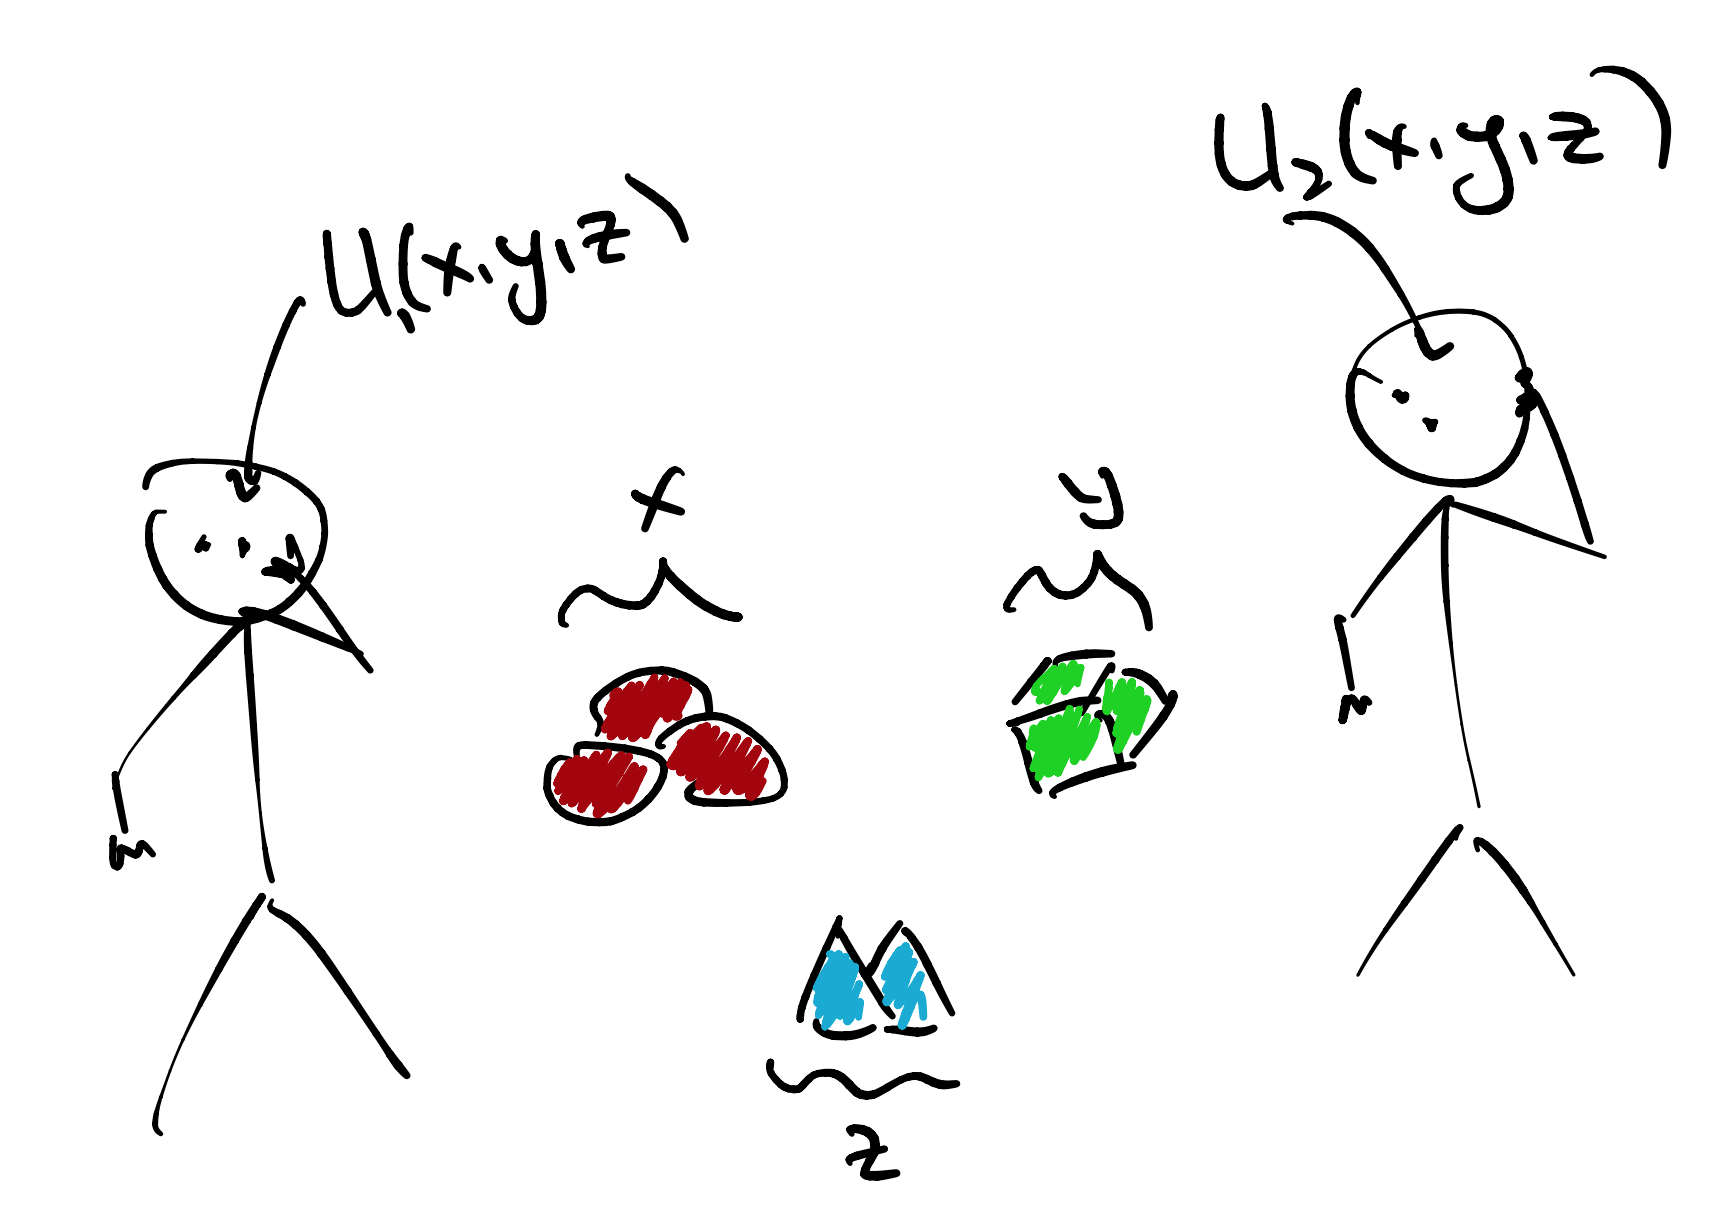
\includegraphics[width=1 \textwidth]{pic2}
\end{figure}

\end{frame}

\begin{frame}{Полезность}

Полезность определена с точностью до монотонного преобразования. Это серьезная проблема, это значит, что модель невозможно толком откалибровать.

Действительно, все ниже перечисленные полезности неразличимы с точки зрения эконометриста. 
\begin{itemize}
\item $x^2 y^3$
\item $2 \log x + 3 \log y$
\item $2 \log x + 3 \log y + 1$
\item $5(2 \log x + 3 \log y) + 1$
\end{itemize}

Необходимо либо мыслить в терминах классов эквивалентности полезностей, либо придумывать что то более подходящее.

\end{frame}

\begin{frame}{Предпочтения}

В (нео классической) модели предпочтений, от агентов требуется, казалось бы, меньше. Они должны в моменте сравнить два портфеля и назвать лучший. Другими словами, они должны озвучить предпочтения.

\end{frame}

\begin{frame}{Предпочтения}

\begin{figure}[hbt]
\centering
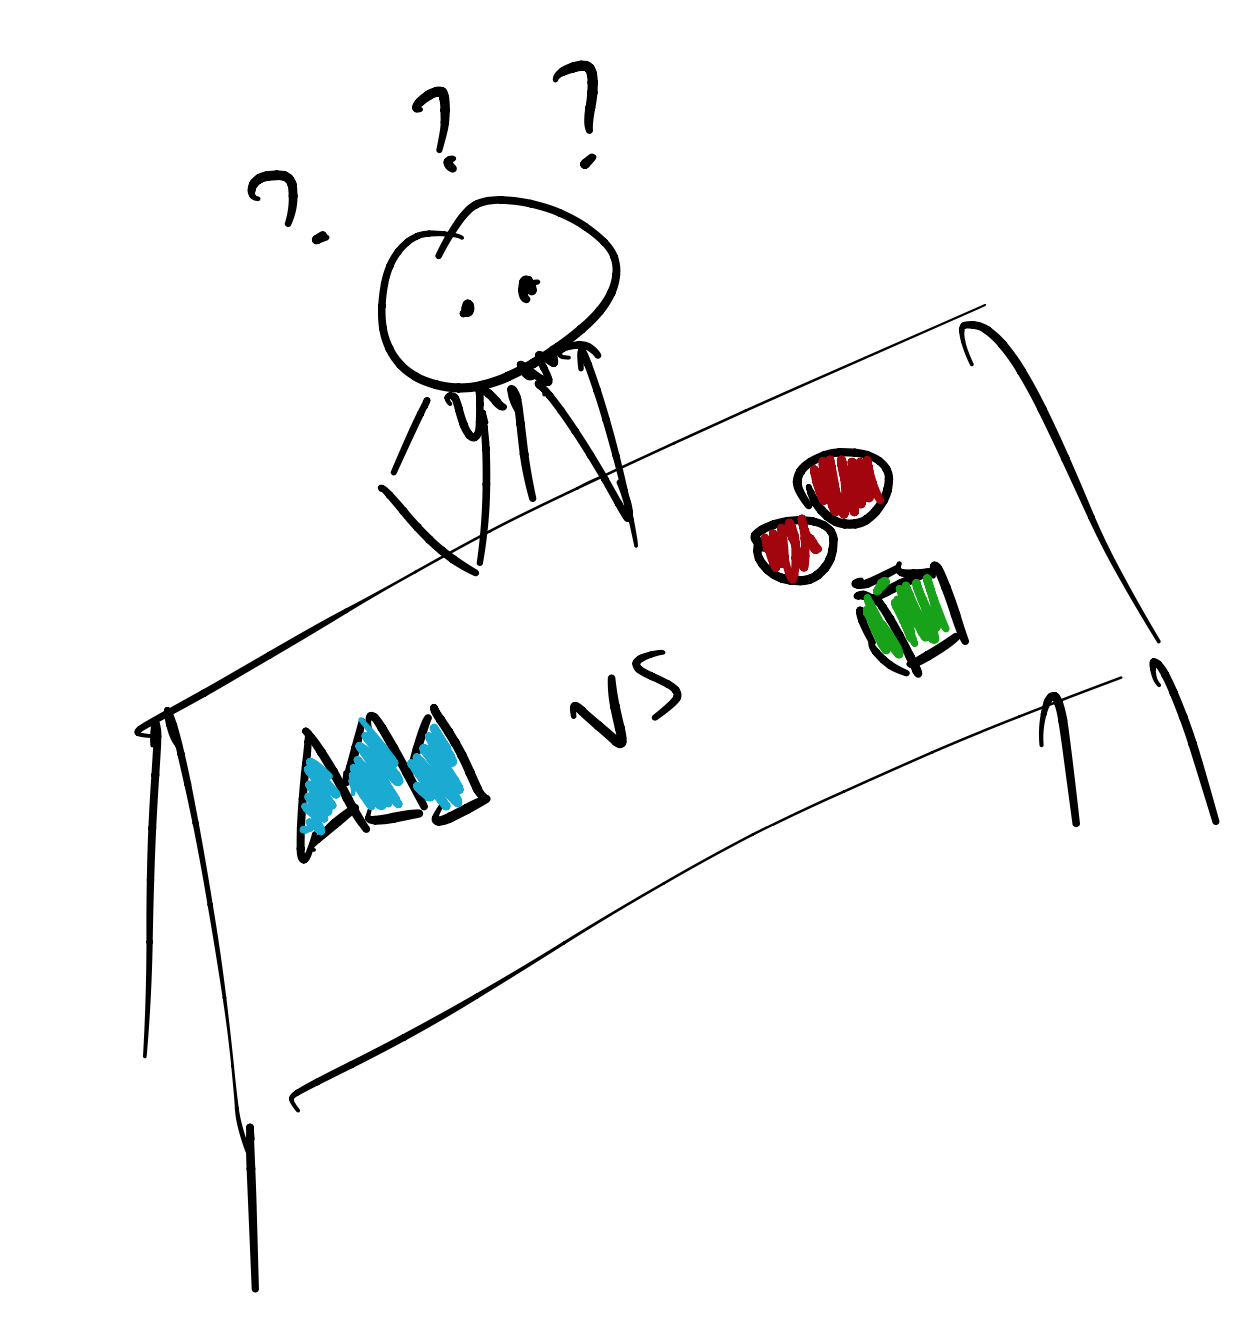
\includegraphics[width=.7 \textwidth]{pic4}
\end{figure}

\end{frame}

\begin{frame}{Предпочтения}

Однако, этот минимализм обманчив. Чтобы оставаться экономическим агентом, они должны помнить все свои выборы, это матрица $n \times n$, где $n$ это число возможных портфелей...

... так уж это проще чем функция? Непонятно

\end{frame}

\begin{frame}{Выбор}

В модели выбора, от агентов требуется принимать решения максимально приближенные к реальности. Вам предлагают меню из: мясо+брокколи+сок, рыба+пиво, рыба+мясо, пиво+сок, брокколи+сок...

И вы просто вычеркиваете то, что вам точно не нравится.

\end{frame}

\begin{frame}{Выбор}

\begin{figure}[hbt]
\centering
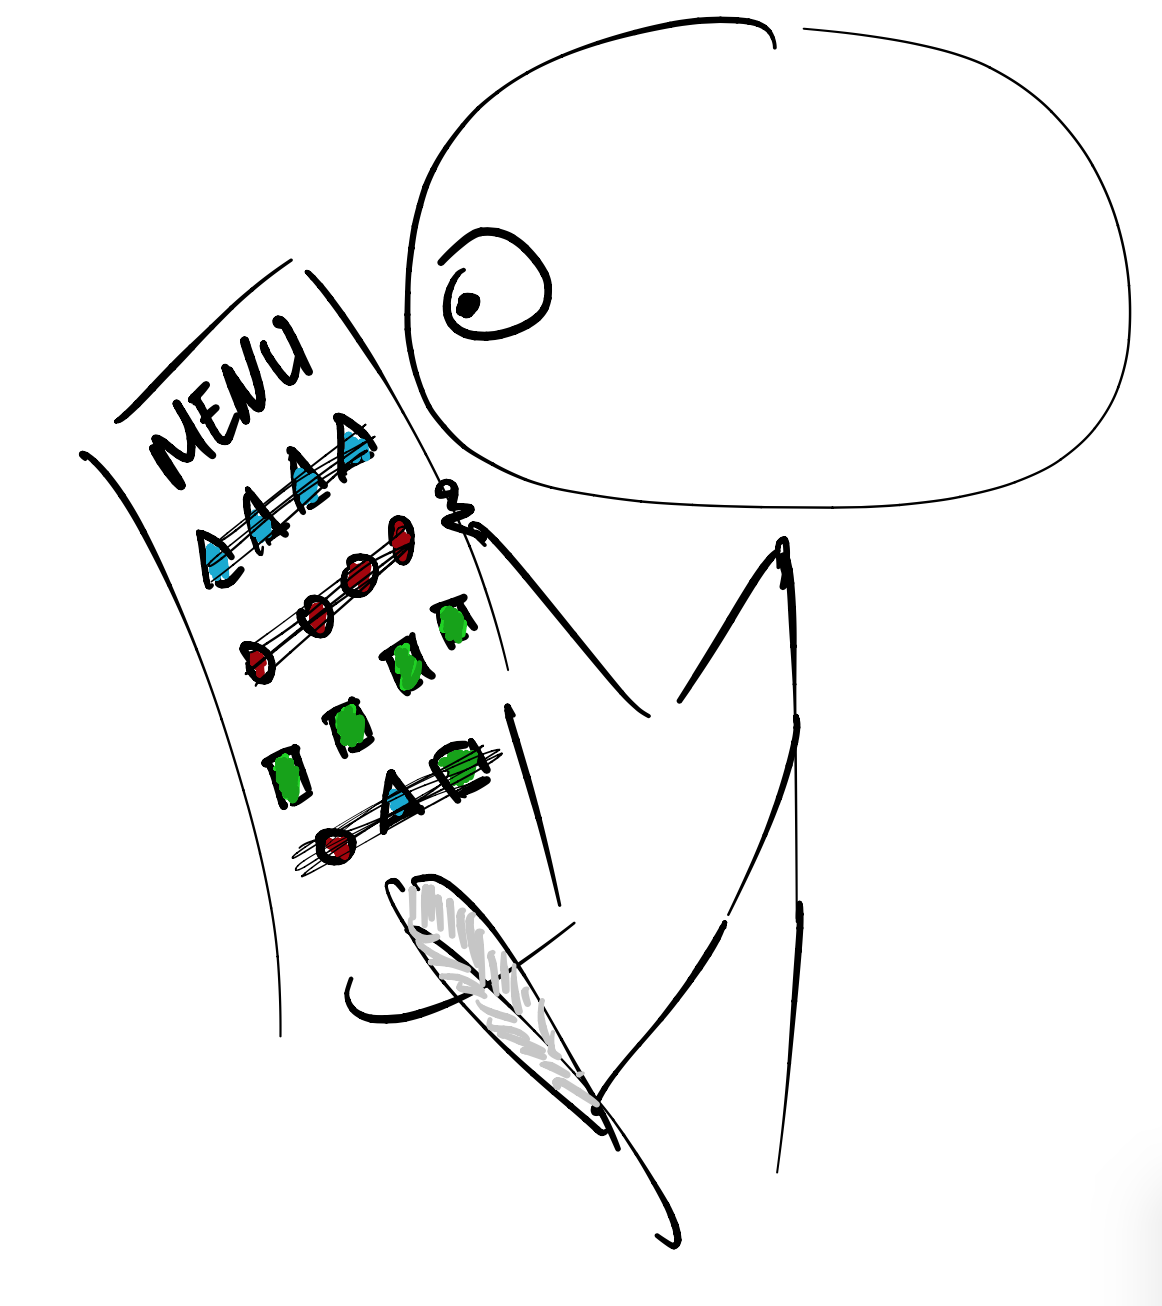
\includegraphics[width=.7 \textwidth]{pic3}
\end{figure}

\end{frame}

\begin{frame}{План на первую половину лекции (2 часа)}

Мы поговорим подробно о первых двух моделях (полезность и предпочтения) и, вскользь о третьей модели (выбор). Большой упор будет сделан на понятия непрерывности и выпуклости.

Затем, мы попробуем отождествить некоторые из этих моделей между собой. В частности, будет обсуждена относительно простая прямая связь между полезностью и предпочтениями.

Вершиной этого блока будет обратная связь между предпочтениями и полезностью, так называемая, Теорема Дебре. После нее надо сделать перерыв.

\end{frame}

\section{Полезность}

\begin{frame}{Полезность}

Модель полезности обладает высоким уровнем абстракции

\begin{itemize}
\item начнем с одного агента
\item товары разделены на $n$ категорий
\item портфель (потр. корзина) это точка в $\mathbb{R}_{+}^{n}$	
\item категории, а также координаты обозначаются $x, y, z...$
\item соответствующие цены обозначаются $p, q, y...$
\item полезность обозначается $U(x,y,z, \ldots)$
\item множество доступных альтернатив $X \subset \mathbb{R}_{+}^{n}$
\end{itemize}

Множество альтернатив будет, как правило, зависеть от цен и, может быть, еще от чего то, например бюджета.


\end{frame}

\begin{frame}{Полезность}

Таким образом, мы может сформулировать модель потребителя как как абстрактную оптимизационную задачу, скажем, для трех товаров:
$$ U(x,y,z, \ldots) \to \max_{(x,y,z, \ldots) \in X}$$
Формально \textbf{классическая  (утилитарная) модель} это пара: множество альтернатив $X \subset \mathbb{R}^n_{+}$ и полезность $U: X \to \mathbb{R}$.

Никаких дополнительных аксиом не требуется.

\end{frame}

\begin{frame}{Пример 1}

У Пети есть 100 рублей. Он может купить яблоки по цене 20 рублей за штуку либо груши по цене 50 рублей за штуку. Петя получает полезность 2 за каждое яблоко и 3 за каждую грушу, но не получает никакой полезности за оставшиеся деньги. 

Попробуем записать это формально:

\begin{itemize}
  \item $X = \{(x, y) \in  \mathbb{N}^2_{+}: 20 x + 50 y \leqslant 100 \}$
  \item $U(x, y) = 2x + 3y$
\end{itemize}

\end{frame}

\begin{frame}{Пример 2}

У Кати есть 24 часа в сутки, из которых она должна как минимум 8 часов поспать, a оставшиеся часы входят в полезность вида Коб-Дуглас с одинаковыми весами, то есть, учеба и вечеринки в полезности умножаются под корнем.

Попробуем записать это формально:

\begin{itemize}
  \item $X = \{(x, y, z) \in  \mathbb{N}^3_{+}: x + y + z \leqslant 24 \}$
  \item $U(x, y, z) = \mathbb{I}(x \geqslant 8)\cdot y^{1/2}z^{1/2}$
\end{itemize}

\end{frame}

\begin{frame}{Пример 3}

У Саши есть 10,000,000 рублей, которые он может вложить в биткойн по курсу 1,000,000:1 или этериум по курсу 1,000,000:2. Саша ожидает, что через год рубль подешевеет на 10\%, биткойн подорожает на 50\% а этериум подорожает на 100\%.

Попробуем записать это формально:

\begin{itemize}
  \item $X = \{(x, y, z) \in  \mathbb{N}^3_{+}: x + 10^6 (y + 2 z) \leqslant 10^7 \}$
  \item $U(x, y, z) = .9 x + 1.5 y + 2 z$
\end{itemize}

\end{frame}

\section{Свойства полезности}

\begin{frame}{Непрерывность}

Мы начнем с двух эквивалентных определений непрерывности.

\begin{definition}
Полезность $U$ \textbf{непрерывна} в $X$, если для любого $x \in X$ множества $L_{+}(x)$ и $L_{-}(x)$ замкнуты, где
\begin{gather*} L_{+}(x) = \{y \in X: U(y) \geqslant U(x)\}\\
 L_{-}(x) = \{y \in X: U(y) \leqslant U(x)\}\end{gather*}
\end{definition}

Описанные выше множества $L_{+}(x)$ (или $L_{-}(x)$) это подмножества допустимых альтернатив, которые не хуже (или не лучше) чем сам $x$. 

Их часто называют \textbf{Лебеговыми множествами}.

\end{frame}

\begin{frame}{Непрерывность}

\begin{figure}[hbt]
\centering
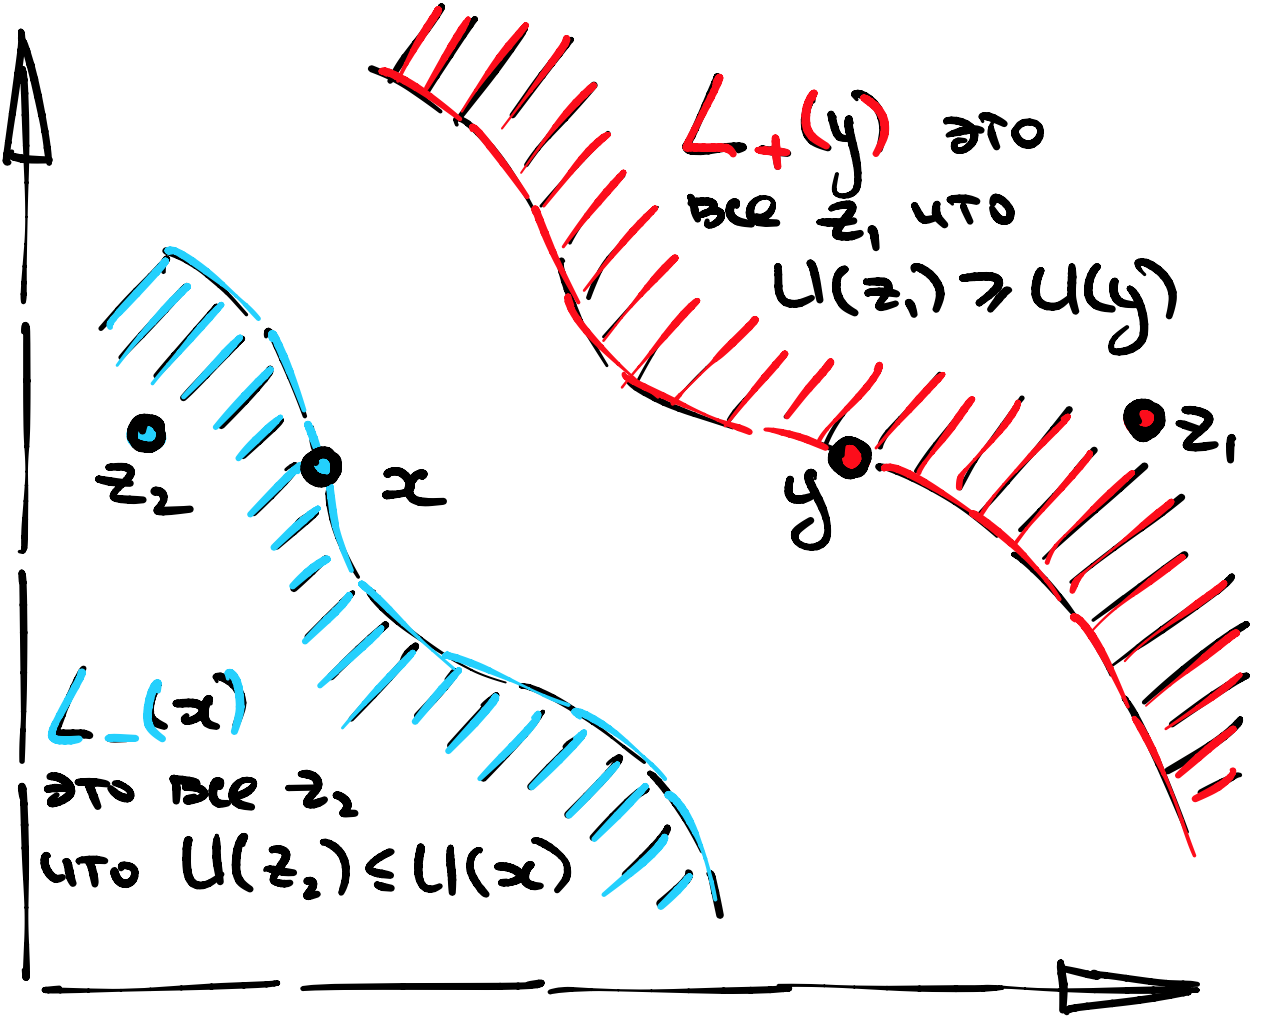
\includegraphics[width=.8 \textwidth]{lebeg_sets.png}
\end{figure}

\end{frame}

\begin{frame}{Непрерывность}

Эквивалентное (но только в Евклидовых пространствах) определение непрерывности можно дать на более знакомом вам с курса мат. анализа языке эпсилон-дельта.

\begin{definition} Полезность $U$ \textbf{непрерывна} в $X$, если для любого $\varepsilon > 0$ существует $\delta >0$ такой что для любых $x, y \in X$: $$ ||x - y|| < \delta \quad \Rightarrow \quad ||U(x) - U(y)|| < \varepsilon.$$	
\end{definition}

Оно абсолютно бесполезно.

\end{frame}

\begin{frame}{Вогнутость}

Следующее важное определение это вогнутость.

\begin{definition}
Полезность $U$ \textbf{вогнута} если для любых $x, y \in X$: 
$$ \forall \alpha \in (0,1): U(\alpha x + (1-\alpha) y)) \geqslant \alpha U(x) + (1-\alpha) U(y)$$
\end{definition}

Грубо говоря, если вы возьмете две точки на поверхности, соответствующая вогнутой полезности, то соединяющая их хорда пройдет "под" поверхностью. 

Другими словами, полезность в усредненной точке меньше чем усредненная полезность.

\end{frame}

\begin{frame}{Вогнутость}

\begin{figure}[hbt]
\centering
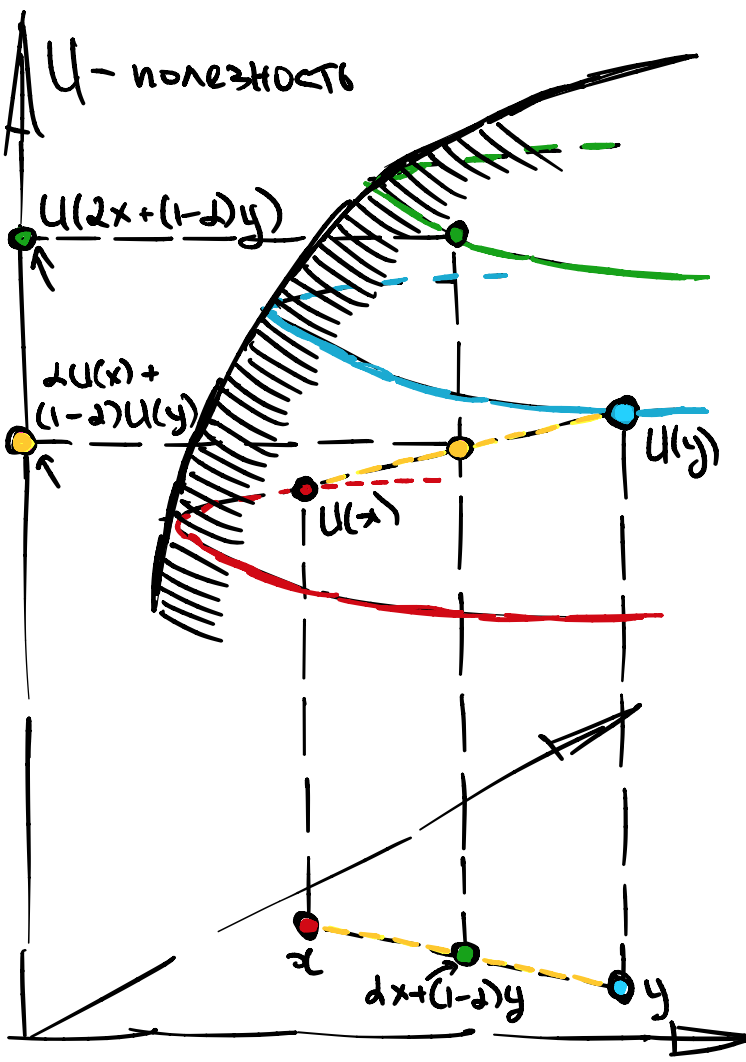
\includegraphics[width=.5 \textwidth]{concave.png}
\end{figure}

\end{frame}

\begin{frame}{Квази вогнутость}

Далее идет определение квази вогнутости.

\begin{definition}
Полезность $U$ \textbf{квази-вогнутa} в $X$, если $\forall x \in X$ множество $L_{+}(x)$ выпукло, то есть, оно содержит все свои хорды. 
\end{definition}

И почти (но не совсем) эквивалентное ему

\begin{definition}
Полезность $U$ \textbf{квази-вогнута} в $X$ если для любых $x, y \in X$ их линейная комбинация не хуже чем худшая из двух:
$$ \forall \alpha \in (0,1): U(\alpha x + (1-\alpha) y)) \geqslant \min(U(x), U(y))$$

\end{definition}

\end{frame}

\begin{frame}{Квази вогнутость}

\begin{figure}[hbt]
\centering
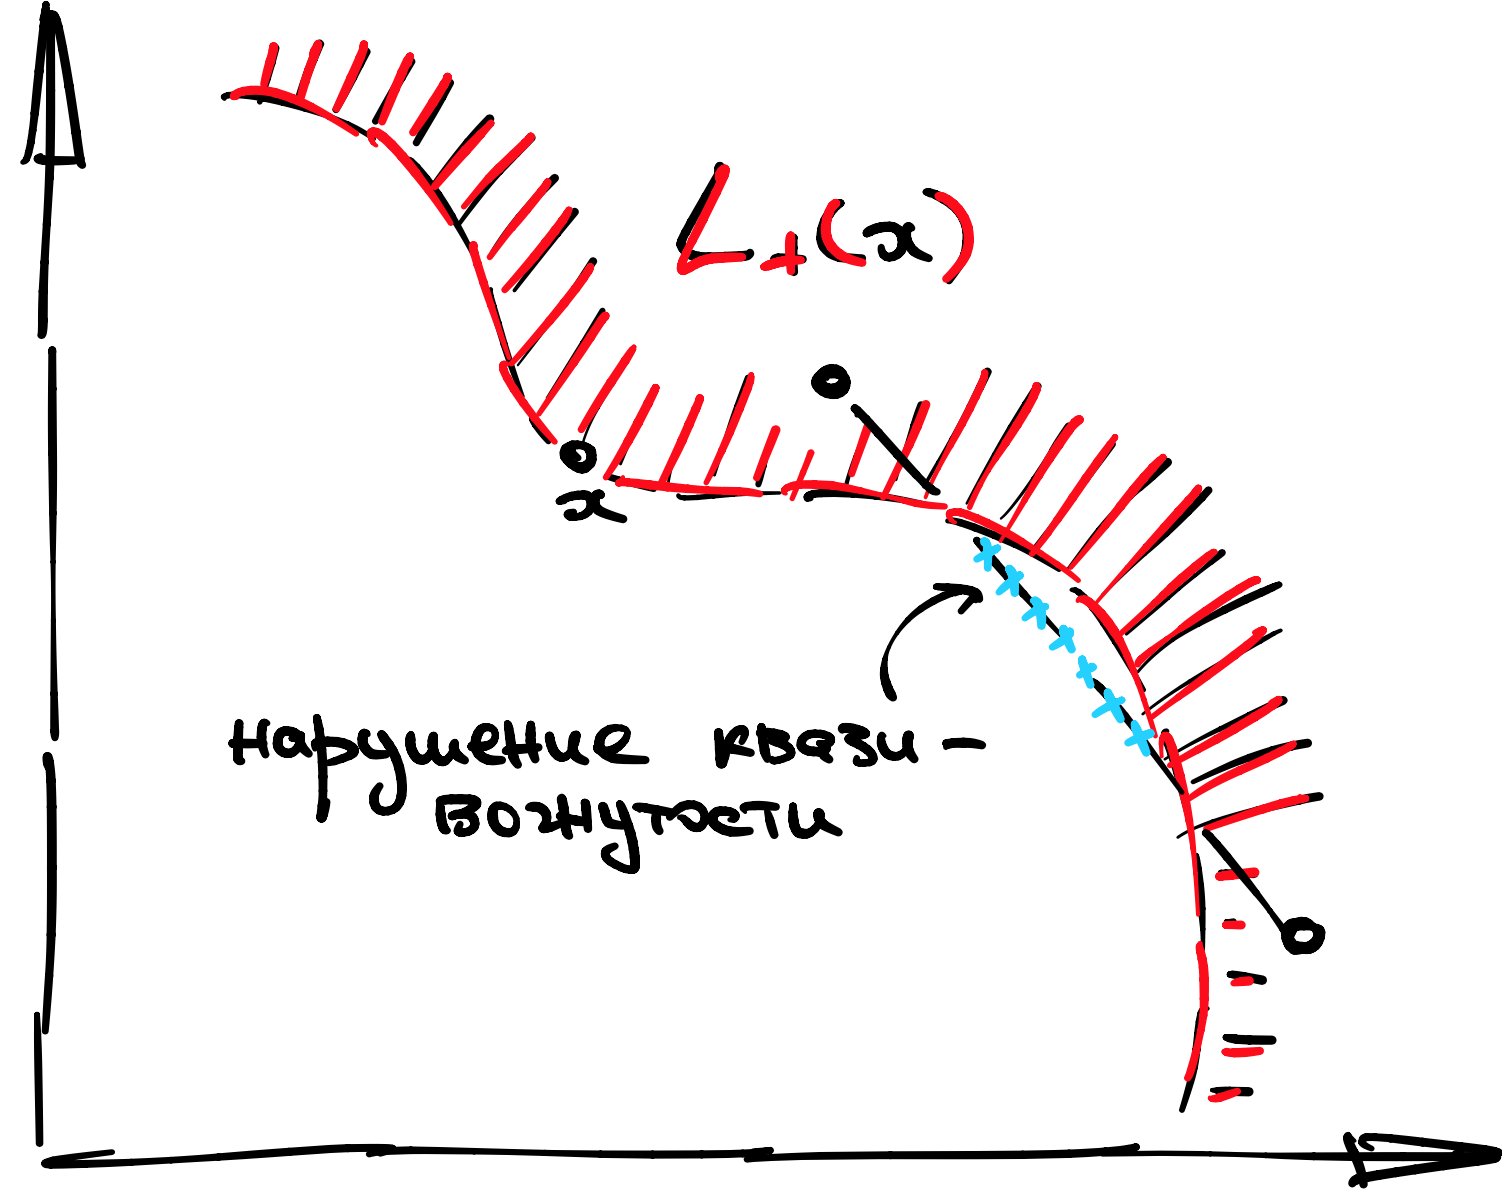
\includegraphics[width=.8 \textwidth]{not_quasi.png}
\end{figure}

\end{frame}

\begin{frame}{Вогнутость против квази вогнутости}

\begin{lemma}
Из вогнутости следует квази-вогнутость, но не наоборот.
\end{lemma}

\begin{proof}
\begin{align*} 
(1) : & \quad U(\alpha x + (1-\alpha) y)) \geqslant \alpha U(x) + (1-\alpha) U(y) \\
(2) : & \quad \alpha U(x) + (1-\alpha) U(y) \geqslant \min (U(x), U(y))\\
(1), (2) \quad \Rightarrow & \quad U(\alpha x + (1-\alpha) y)) \geqslant \min (U(x), U(y))
\end{align*}
\end{proof}

P.S. Иногда я буду делать приставку ''строго'', это значит что либо множество строго выпукло, либо неравенство строгое. Смотрите на контекст.

\end{frame}

\section{Критика классической модели}

\begin{frame}{Неоднозначность полезности}

Для любого строго монотонного преобразования $\varphi$, две полезности: $U(x)$ и $\varphi(U(x))$ производят идентичное поведение у потребителей.  

Довольно легко генерировать примеры идентичных функций используя такие монотонные преобразования как $\varphi(z) = z + c, cz , \log z$.
\begin{align*}
& x^2y^3,\\
& 2\log x + 3\log y,\\
& 2\log x + 3\log y + 1,\\
& 2(2\log x + 3\log y) + 1.
\end{align*}
Все выше перечисленные полезности эквивалентны.
\end{frame}

\begin{frame}{Неоднозначность вогнутости}

Вогнутость легко ломается при монотонных преобразованиях

\begin{lemma}
Если $U(x)$ вогнута, то $\varphi(U(x))$ квази-вогнута для любого строго монотонного преобразования $\varphi$. 
\end{lemma}

Чтобы придумать доказательство, достаточно знать следующие свойства монотонных преобразований:
 \begin{align*}
U(x) \leqslant U(y) \quad \Leftrightarrow \quad \varphi(U(x)) \leqslant \varphi(U(y))\\
U(x) \geqslant U(y) \quad \Leftrightarrow \quad \varphi(U(x)) \geqslant \varphi(U(y))\\
\min(\varphi(U(x)), \varphi(U(y))) = \varphi(\min(U(x),U(y)))
\end{align*}

Попробуйте теперь написать доказательство самостоятельно.

\end{frame}

\begin{frame}{Неоднозначность вогнутости}

В отличие от вогнутости, квази вогнутость сохраняется при монотонных преобразованиях.

Это верно хотя бы потому, что одно из двух определений вообще никак не опирается на форму полезности, а только на форму Лебеговых множеств.

\begin{lemma}
Если $U(x)$ квази-вогнута, то $\varphi(U(x))$ тоже квази-вогнута для любого строго монотонного преобразования $\varphi$. 
\end{lemma}

Это делает ее гораздо более удобной чем просто вогнутость.

\end{frame}

\section{Предпочтения}

\begin{frame}{Предпочтения}

Модель предпочтений еще более абстрактна

\begin{itemize}
\item снова один агент
\item товары разделены на $n$ категорий
\item портфель (потр. корзина) это точка в $\mathbb{R}_{+}^{n}$	
\item категории, а также координаты обозначаются $x, y, z...$
\item множество доступных альтернатив $X \subset \mathbb{R}_{+}^{n}$
\end{itemize}

Однако вместо полезности $U: X \to \mathbb{R}$ у агента в голове зашито бинарное предпочтение $\succcurlyeq: X^2 \to \{0,1\}.$ Что это значит?

\end{frame}

\begin{frame}{Предпочтения}

Проще всего визуализировать бинарное отношение на множестве альтернатив малой размерности, например 3.
$$
\begin{array}{c|ccc}
 \succcurlyeq & x & y & z\\
\hline
x & 1 & 1 & 0 \\
y & 0 & 1 & 1\\
z & 0 & 1 & 0
\end{array}
$$

$x \succcurlyeq y$ означает что $(x,y) \mapsto 1$.

$x \preccurlyeq y$ означает что $(y,x) \mapsto 1$.

Формально, бинарное отношение это любое расположение ноликов и единичек внутри матрицы.

\end{frame}

\begin{frame}{Предпочтения}

Для простоты, вводятся дополнительные обозначения:

$x \sim y$ означает что $x \succcurlyeq y$ и $x \preccurlyeq y$.

$x \succ y$ означает что $x \succcurlyeq y$ но не $x \sim y$.

$x \prec y$ означает что $x \preccurlyeq y$ но не $x \sim y$.

Получаются пять интуитивных отношений сильного, слабого предпочтений и безразличия.

Однако, какие попало матрицы писать не стоит.

\end{frame}

\begin{frame}{Предпочтения}

Поскольку у бинарного отношения есть экономическая интерпретация, это накладывает на него определенные ограничения, называемые \textbf{аксиомами рациональности}.

\begin{definition}
Предпочтения $\succcurlyeq$	\textbf{рациональны}, если
\begin{itemize}
\item для любыx $x, y \in X$, хотя бы $x \succcurlyeq y$ либо $y \succcurlyeq x$.
\item для любой $x \in X$, всегда верно что $x \sim x$
\item для любыx $x, y, z \in X$: 
$$x \succcurlyeq y, y \succcurlyeq z \quad \Rightarrow \quad x \succcurlyeq z$$
\end{itemize}
\end{definition}
Последнее свойство - самое важное и называется \textbf{транзитивностью}. 

\end{frame}

\begin{frame}{Предпочтения}

Рациональность накладывают структуру на то как может заполняться матрица. 
$$ 
\begin{array}{c|ccc}
 \succcurlyeq & x & y & z\\
\hline
x & * & * & * \\
y & 0 & * & 1\\
z & 0 & 1 & *\\
\end{array}
$$
Попробуйте до-заполнить следующую матрицу так, чтобы предпочтения были рациональными.

\end{frame}

\section{Свойства предпочтений}

\begin{frame}{Предпочтения}

Практически копипастой мы определяем непрерывность предпочтений.

\begin{definition}
Предпочтения $\succcurlyeq$ \textbf{непрерывны} в $X$, если для любого $x \in X$ множества $L_{+}(x)$ и $L_{-}(x)$ замкнуты, где
$$L_{+}(x) = \{y \in X: U(y) \geqslant X\}, \quad L_{-}(x) = \{y \in X: U(y) \leqslant X\}$$
\end{definition}

И совершенно аналогично мы переносим квази-вогнутость в мир предпочтений...

\end{frame}

\begin{frame}{Предпочтения}

... однако, вопреки логике, термин квази-ВОГНутости полезности превращается в ВЫПУклость предпочтений.

\begin{definition}
Предпочтения $\succcurlyeq$ \textbf{выпуклы} в $X$, если $\forall x \in X$ множество $L_{+}(x)$ выпукло, то есть, оно содержит все свои хорды. 
\end{definition}

Парадокс в том, что вогнутые полезности квази-вогнуты, которые, в свою очередь, ассоциированы с выпуклыми предпочтениями. 

А выпуклые полезности (которые еще надо отыскать) с выпуклыми предпочтениями вообще никак не связаны и даже прямо противоположны им. 

\end{frame}

\end{document}